\chapter{Wand \textit{multi-threaded}}
\label{cap:wand}

Dado que el método WAND \citep{Broder:2003} consiste es el método del estado del arte ocupado hoy en día por los motores de búsqueda, en esta investigación se asume un sistema que usa este método para obtener eficientemente los mejores K documentos a una transacción de lectura. Este algoritmo usa un \textit{ranking} basado en una evaluación de dos niveles. En el primer nivel, este usa una cota superior (\textit{upper bound}) al puntaje de cada documento para intentar descartarlos eficientemente. En el segundo nivel se computa el puntaje real de los documentos que pasa el primer nivel. Se utiliza una estructura de datos llamada \textit{heap} que va guardando el conjunto de los mejores K documentos hasta un determinado instante. El menor puntaje de este conjunto es usado como umbral (\textit{threshold}) para las evaluaciones del primer nivel, de esta forma se descarta rápidamente documentos que no pueden ser parte del conjunto final de los \textit{top-K} documentos. Esto permite un eficiente y a la vez seguro proceso de descarte que asegura que en el resultado final se encontrará el conjunto correcto y no se perderán documentos relevantes.

Existen dos formas de implementar Wand \textit{multithreaded}. Una de ellas es usando \textit{heaps} locales (LH), es decir, un \textit{heap} por hilo de ejecución (\textit{thread}) y el otro es usando \textit{heaps} compartidos (SH). El estudio en \citep{Rojas:2013} se muestra indicios que el esquema SH es generalmente más eficiente. Logrando rápidamente un óptimo valor para el threshold, el esquema SH posee las siguientes ventajas: (1) Se puede reducir el número de calculo de puntajes completos y (2) se ejecutan pocas operaciones de actualización del heap (reduciendo el número de \textit{locks} que se hace a la estructura de dato). A continuación se presenta el diseño llevado a cabo para ambos esquemas.

\section{Block max wand}
Recordar que en el método de Wand para descartar documentos y encontrar un documento que potencialmente podría estar en el conjunto \textit{top-K}, lo que se hace es usar los \textit{upper bounds} globales de cada lista, es decir, la máxima contribución (puntaje o \textit{score}) de algún documento de la lista invertida. Además, Wand tradicional es una estrategia DAAT, por lo que por cada lista invertida ocupa un puntero al documento actual que se desea evaluar. Además, usa un método que recibe como entrada un identificador del documento $docID$ y una lista invertida $L$, y retorna el primer $docID'$ que sea mayor o igual al documento $docID$. A esto se le conoce como movimiento de puntero profundo (\textit{deep pointer movement}) debido a la razón que generalmente implica una descompresión del boque en el que se encuentra el documento.

Sin embargo, como se dijo anteriormente en \ref{marco:bmw}, usando solo las máximas contribuciones por cada bloque no hará que el método funcione correctamente, puesto que hará que eventualmente se pierdan documentos que podrían estar en el conjunto final de los mejores $K$ documentos. Como ahora se tiene las máximas contribuciones por cada bloque, BMW utiliza otra función la cual recibe como parámetro un identificador de documento $docID$ y una lista invertida. Lo que se hace es mover el puntero actual al correspondiente bloque donde eventualmente se debería encontrar el documento $docID$. A esta función se le conoce como movimiento de puntero superficial (\textit{shallow pointer movement}), por la razón que no involucra una descompresión de bloque. Se debe notar que para que esta función trabaje correctamente se requiere tener almacenada las fronteras de cada uno de los bloques de las listas invertidas.

BMW utiliza dos principales ideas en su diseño: (1) Se usa los \textit{upper bounds} globales para determinar un pivote candidato (como en Wand tradicional), para luego usar los \textit{upper bounds} locales para determinar si es que el pivote candidato es un pivote real o no, y (2) Se intenta siempre utilizar \textit{shallow pointer movement} por sobre \textit{deep pointer movement}.

En el Algoritmo \ref{alg:bmw} se puede apreciar cómo el método \textit{Block-Max-Wand} trabaja. Recordar que todas las listas invertidas poseen un puntero al documento actual que se desea evaluar (\textit{currentDoc}). Lo primero que se hace es ordenar en orden creciente las listas invertidas de acuerdo a su correspondiente \textit{currentDoc}. La función \textit{findPivot()} es la misma que se utiliza en el método Wand tradicional (\ref{marco:wand}), se itera sobre las listas invertidas y se retorna la posición de la lista en donde se cumple que la suma de los \textit{upper bounds} globales es mayor al \textit{threshold} ($\theta$). Luego la función \textit{NextShallow()} se encarga de avanzar los punteros de las listas invertidas al inicio del bloque que debería contener el documento $d$. Posteriormente la función \textit{isRealPivot()} verifica si es que el pivote $p$ encontrado es un pivote real o no, para cada una de las listas desde la posición $0$ hasta la posición $p$, se suma los \textit{upper bounds} de los bloques en donde se encuentran los punteros (recordar que con \textit{NextShallow()} los punteros de las listas quedaron apuntando a los bloques en donde se debería encontrar el documento $d$), si la suma es mayor al threshold entonces retorna verdadero, de lo contrario retorna falso. El método \textit{scoreDoc()} calcula el puntaje del documento que se le pasa por parámetro. 

Cuando el método se da cuenta que $p$ no es un pivote real, lo que se hace es buscar un nuevo candidato a través de la función \textit{getNewCandidate()}, la cual hace avanzar los punteros de las listas invertidas hasta el bloque siguiente que contenga el mínimo $docID$. Para ver explicar de mejor manera esta idea se presenta la Figura \ref{fig:getNewCandidate}, aquí se puede ver que el documento $4868$ es el pivote, cuando este documento no es un pivote real (la función \textit{isRealPivote} retorna falso), lo que se hará es escoger un documento $d'$ tal que $d = min(d1,d2,d3,d4)$ en donde $d1,d2,d3$ son la frontera del bloque actual más uno (inicio del bloque siguiente) y $d4$ es el \textit{currentDoc} de la cuarta lista. Notar que para hacer un descarte seguro de documentos, siempre se debe incluir a la elección del nuevo candidato el \textit{currentDoc} de la lista inmediatamente siguiente a la lista pivote (en este caso 9009).  

\begin{figure}[!th]
\centering
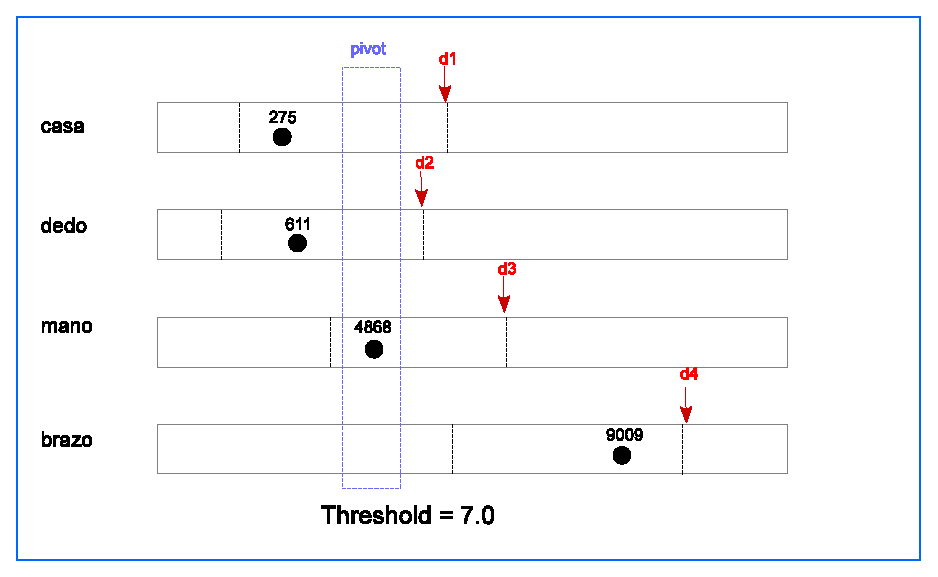
\includegraphics[scale=.75]{images/get_new_candidate.eps}
\caption{Ejemplo de cómo opera la functión getNewCandidate()}
\label{fig:getNewCandidate}
\end{figure}%y


\begin{algorithm}[!th]
\caption{\em $BMW(\theta, L, docID)$: Block Max Wand}
\label{alg:bmw}
\begin{algorithmic}[1]
\REQUIRE Un \textit{threshold} $\theta$, listas invertidas $L$ de los términos en la consulta
\ENSURE $docID$, si existe un documento $docID$ tal que $score(docID)$ $\geq$ $\theta$. de lo contrario END-OF-FILE
\WHILE {true}
	\STATE $Sort(L);$
	\STATE $p = findPivot(L,\theta);$
	\STATE $d = L[p] \rightarrow currentDoc;$
	\IF {$d == $ END-OF-FILE}
  		\STATE $break;$
	\ENDIF
		
	\FOR {$ i = 0...p $}
		\STATE $NextShallow(d, L[i]);$
	\ENDFOR
	
	\IF {$isRealPivot(\theta, p);$}
		\IF {$L[0] \rightarrow currentDoc == d$}
			\STATE $scoreDoc(d, p);$
			\FOR {$ i = 0...p $}
				\STATE $Next(d + 1, L[i]);$
			\ENDFOR
		\ELSE
			\WHILE {$List[p - 1] \rightarrow currentDoc == p $}
				\STATE $p = p - 1;$			
			\ENDWHILE
			
			\FOR {$ i = 0...p $}
				\STATE $Next(d, L[i]);$
			\ENDFOR
			
		\ENDIF		
	\ELSE	
		\STATE $d' = getNewCandidate();$
		\FOR {$ i = 0...p $}
			\STATE $Next(d', L[i]);$
		\ENDFOR
	\ENDIF
	
\ENDWHILE

\end{algorithmic}
\end{algorithm}

\section{Wand con heaps locales}
En el esquema LH, cada \textit{thread} procesa una porción del índice invertido mientras mantiene un \textit{heap} local con los mejores $K$ documentos que el específico hilo de ejecución ha encontrado hasta ahora. Al final del proceso, los resultados deben ser reunido en un solo conjunto final global. Los resultados en \citep{Rojas:2013} muestran que el esquema LH es más eficientes para aquellas transacciones que toman poco tiempo en ser resueltas. En la Figura \ref{fig:wand-heap-local} se muestra el esquema de ejecución para \textit{heaps} locales explicado anteriormente. 

\begin{figure}[!ht]
\centering
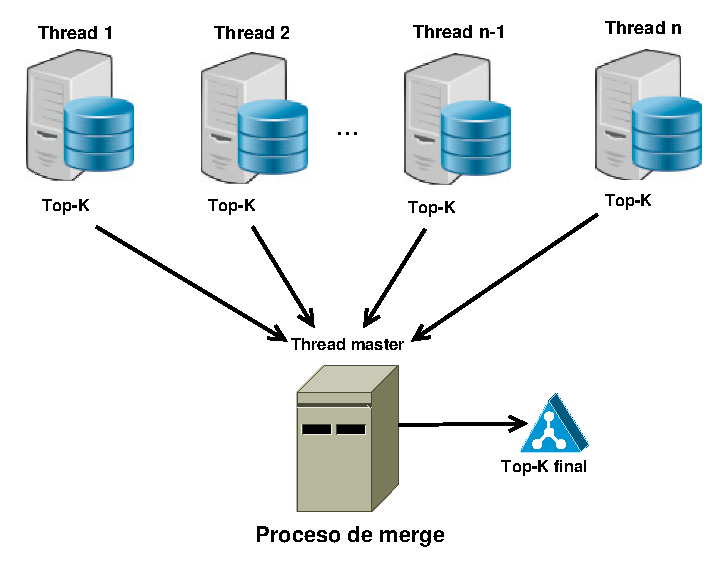
\includegraphics[scale=.75]{images/wand_heaps_locales.eps}
\caption{Esquema de ejecución de algoritmo WAND con heaps locales}
\label{fig:wand-heap-local}
\end{figure}

El diseño aplicado para implementar el esquema LH se puede ver en la Figura \ref{fig:TopKMultiThreadWandOperatorLocal}. La clase principal es la TopKMultiThreadWandOperatorLocal, que es la encargada de controlar el paralelismo en la resolución de las transacciones. Para explicar de mejor manera cada una de las clases involucradas en la implementación, se presenta el siguiente diccionario de datos.

\begin{figure}[!ht]
\centering
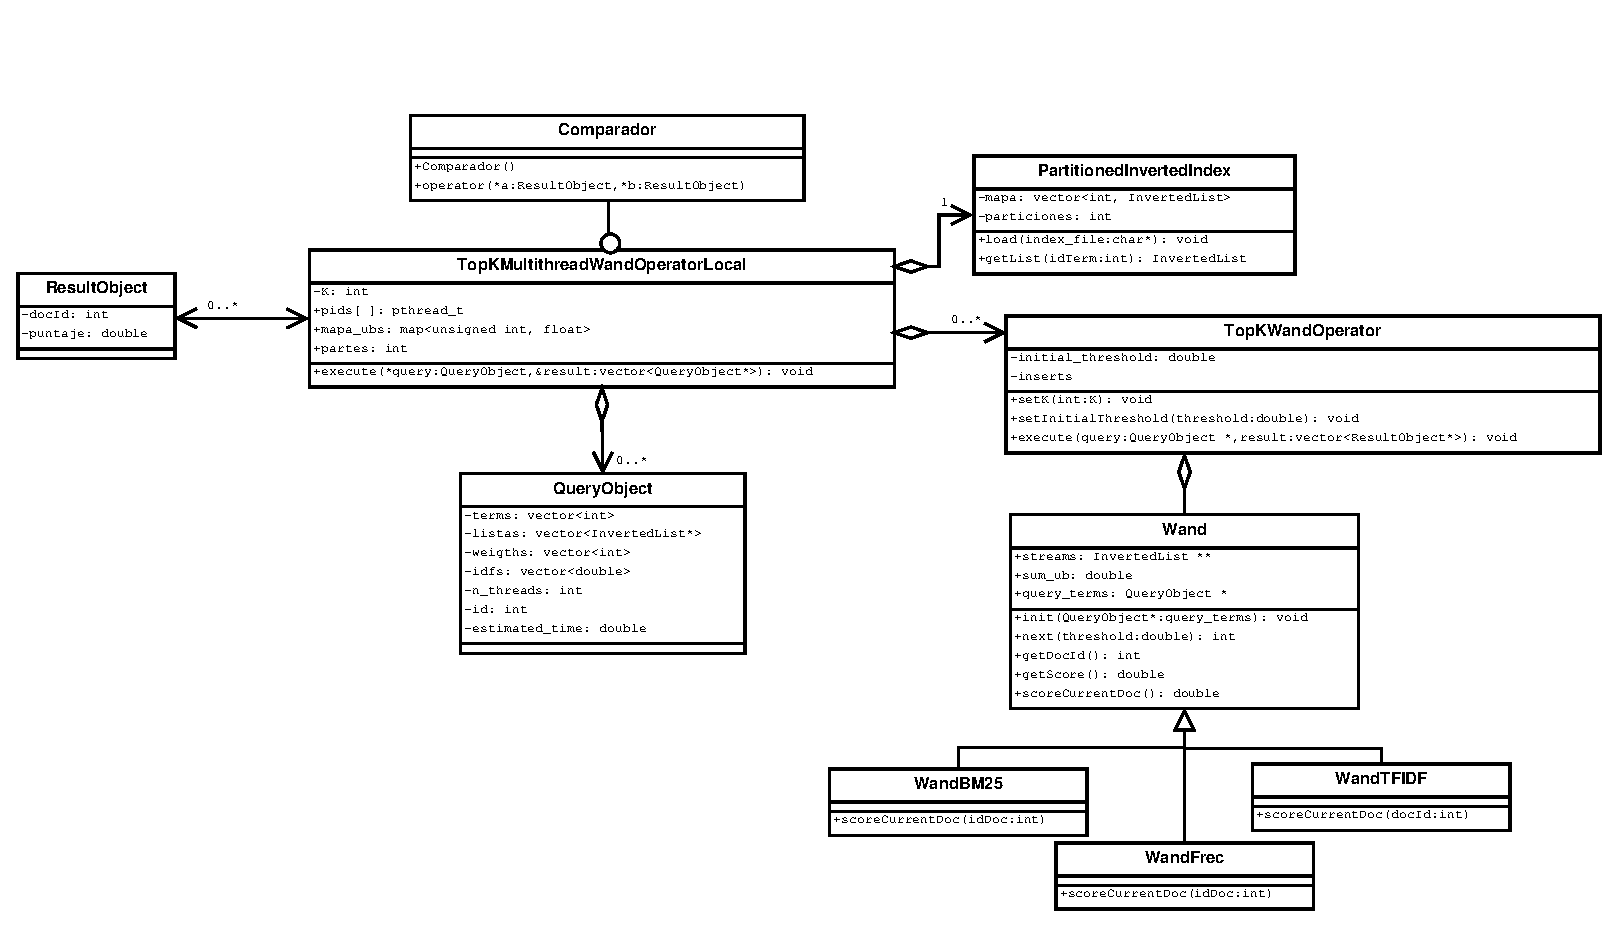
\includegraphics[scale=.75]{images/TopKMultiThreadWandOperatorLocal.eps}
\caption{Diagrama de clases para el esquema LH}
\label{fig:TopKMultiThreadWandOperatorLocal}
\end{figure}

\begin{list}{}{}
	\item \textbf{TopKMultiThreadWandOperatorLocal}. Clase encargada de devolver los mejores K documentos para una query dada. Si es que la query debe ser resuelta en forma paralela, esta clase además debe controlar el paralelismo que se produce en la resolución de ésta, inicializando las variables correspondientes para lanzar los hilos de ejecución y luego escogiendo los mejores documentos desde todos los heaps creados por los diferentes threads (proceso de merge). En esta clase se define un mapa que asocia cada término del índice invertido con el puntaje del mejor documento en esa lista invertida (upper bound de la lista invertida) y además se define cuántos documentos se van a retornar al final del proceso (atributo K). El método execute inicializa las variables locales para los diferentes threads, posteriormente hace el llamado al método \emph{thread-execute} (en el cual se llevará a cabo la resolución de la transacción de lectura en forma paralela), finalmente se toman los resultados parciales de cada uno de los hilos de ejecución y se ejecuta el proceso que mezcla los resultados, retornando solo los mejores K documentos. 
	
	\item \textbf{PartitionedInvertedIndex}. Clase que tiene la tarea de almacenar el índice invertido y extraer desde aquí las listas invertidas de documentos para cada uno de los términos de las transacciones de lectura. El almacenamiento el índice se lleva a cabo mediante un mapa cada término su lista invertida correspondiente y para la extracción de estas listas se usa el método getList.
	
	\item \textbf{TopKWandOperator}.  Cada thread tendrá su propio objeto TopKWandOperator encargado de obtener los mejores K documentos. El cálculo de este conjunto se realiza en el método execute con la ayuda de un objeto de tipo Wand asociado.
	
	\item \textbf{Wand}. Clase que controla la lógica del algoritmo wand. Lleva a cabo el proceso de inserción de documentos en el heap y todo lo que esto conlleva. Existen diferentes tipos de objetos Wand que se pueden utilizar, entre ellos están WandBM25, WandFrec y WandTFIDF, donde la única diferencia entre ellos es el método de que calcula el puntaje de cada documento. Por ejemplo, WandBM25 utiliza BM25 (citar) y WandTFIDF utiliza tf-idf (citar también). 
	
	\item \textbf{ResultObject}. Clase que se utiliza para guardar los mejores K documentos.
	
	\item \textbf{QueryObject}. Clase que representa una transacción de lectura. Está constutuída sus términos,  las respectivas listas invertidas y pesos de cada uno de ellos, la cantidad de threads con los cuales se resolverá dicha transacción y el tiempo estimado de procesamiento (este tiempo se predice al momento de resolver la query).

\end{list}




\section{Wand con heap compartido}
\label{scheduling:whc}
En el esquema SH cada thread procesa una porción del índice. Sin embargo, ahora un solo heap es creado y accedido por todos los threads. En este caso no se requiere de mezclar los resultados y el proceso de descarte tiende a ser más eficiente porque los documentos con mayor puntaje tienden a estar en el heap. Acceder al heap debe ser controlado por un lock o algún método similar que garantice el acceso exclusivo de los threads al heap. Este esquema es más eficiente que el LH en queries que toman mayor tiempo en ser resueltas.

El diseño implementado para este esquema posee como clase principal a TopKMultiThreadWandOperatorLocks y difiere del modelo implementado para el esquema LH en el sentido que ahora se debe controlar el acceso concurrente a los datos compartidos como el heap y el threshold. A continuación se presenta el diccionario de datos del esquema SH mostrado en la Figura \ref{fig:TopKMultiThreadWandOperatorLocks}.

\begin{figure}[!ht]
\centering
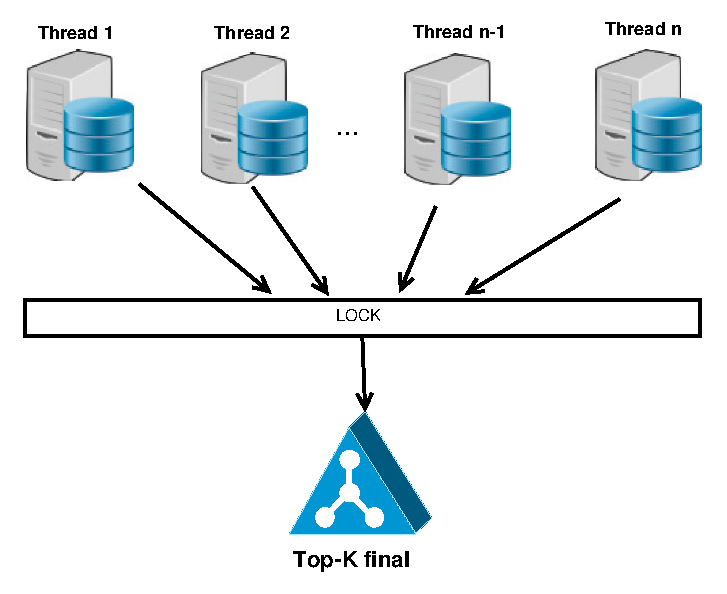
\includegraphics[scale=.75]{images/wand_heaps_compartido.eps}
\caption{Esquema de ejecución de algoritmo WAND con heap compartido}
\label{fig:wand-heap-compartido}
\end{figure}

\begin{list}{}{}
	\item \textbf{TopKMultiThreadWandOperatorLocks}. Clase encargada de inicializar las variables compartidas y de lanzar los threads requeridos para procesar la transacción de lectura.
	
	\item \textbf{WandThreadData}. Clase anidada a TopKMultiThreadWandOperatorLocks que contendrá todas las variables compartidas para el procesamiento de las consultas. Dentro de los atributos más importantes destaca el mutex utilizado para controlar el acceso al heap compartido y además al threshold (en este esquema es un threshold global y compartido a todos los threads).
	
	\item \textbf{Wand}. Al igual que en el esquema anterior, esta clase se encarga de llevar a cabo el proceso de inserción de documentos en el heap y de las actualizaciones del threshold. El método scoreCurrentDoc es el encargado de entregarle un puntaje a cada documento y dependerá de qué tipo de Wand se este utilizando (BM25, WandFrec, WandTFIDF). 

	\item \textbf{PartitionedInvertedIndex}. Clase encargada de almacenar el índice invertido. Posee un método llamado getList que recibe como parámetro el identificador de un documento y retorna la lista invertida asociada. 

\end{list}

\begin{figure}[!ht]
\centering
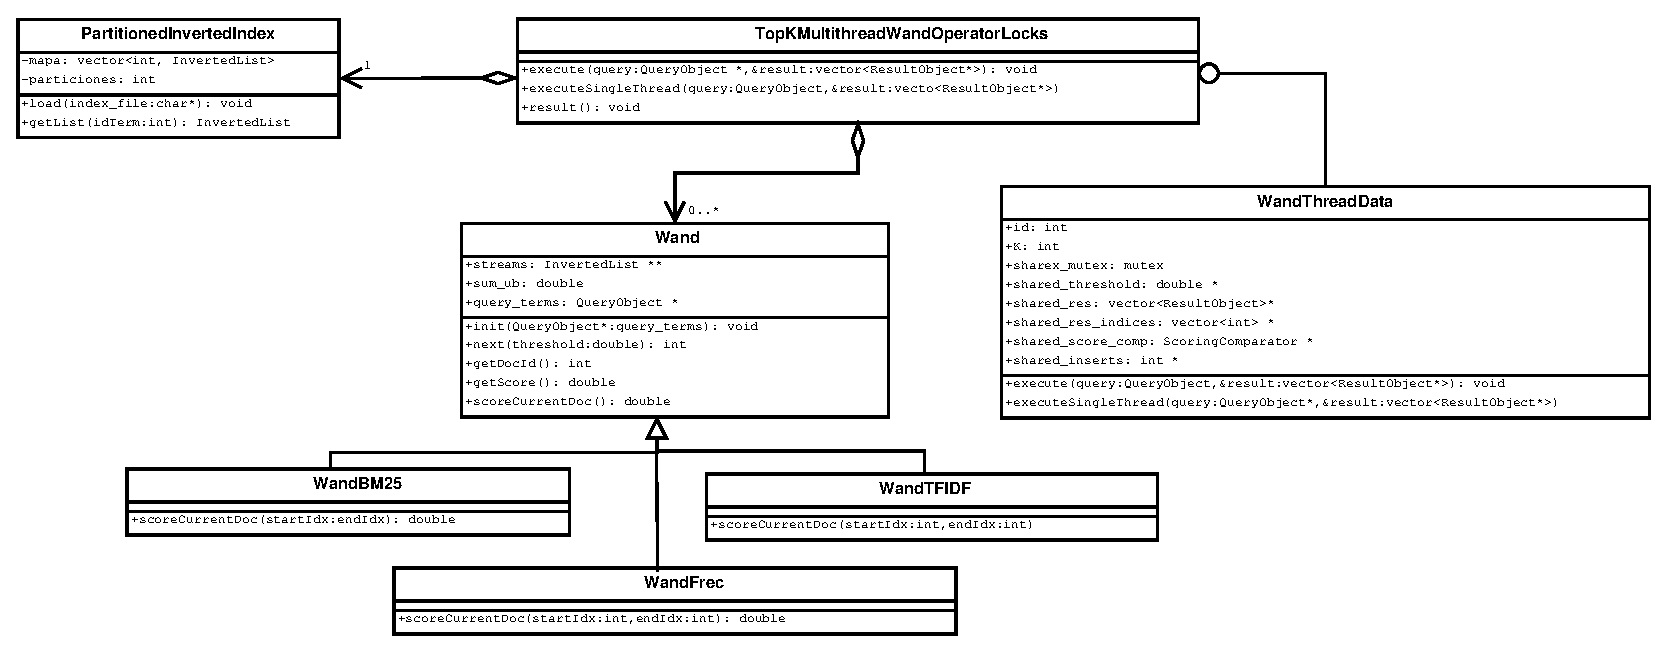
\includegraphics[scale=.75]{images/TopKMultiThreadWandOperatorLocks.eps}
\caption{Diagrama de clases para el esquema SH}
\label{fig:TopKMultiThreadWandOperatorLocks}
\end{figure}
